\section{B-Link-Tree}\label{section:b-link-tree}

Previous approaches include locking a subtree of highest affected node \cite{samadi1976b}, which, albeit straightforward, reduced concurrency. To alleviate the bottleneck without risking inconsistency, \textit{B-Link-Tree} relaxes the definition of B$^+$Trees. As explained by Graefe \cite{goetz-tech}:

\begin{definition}
  B-Link-Tree is a B$^+$Tree with following properties:
  \begin{enumerate}
    \item Each node $x$ has additional attributes:
          \begin{itemize}
            \item $x.sibling$, a pointer to a right sibling node at the same level,
            \item $x.highkey$, the upper bound of all keys found in the subtree rooted by $x$ (every key found in $x$ is less then $x.highkey$).
          \end{itemize}
    \item Does not require locks nor latches for reading.
  \end{enumerate}
\end{definition}

\begin{figure}[H]
  \centering
  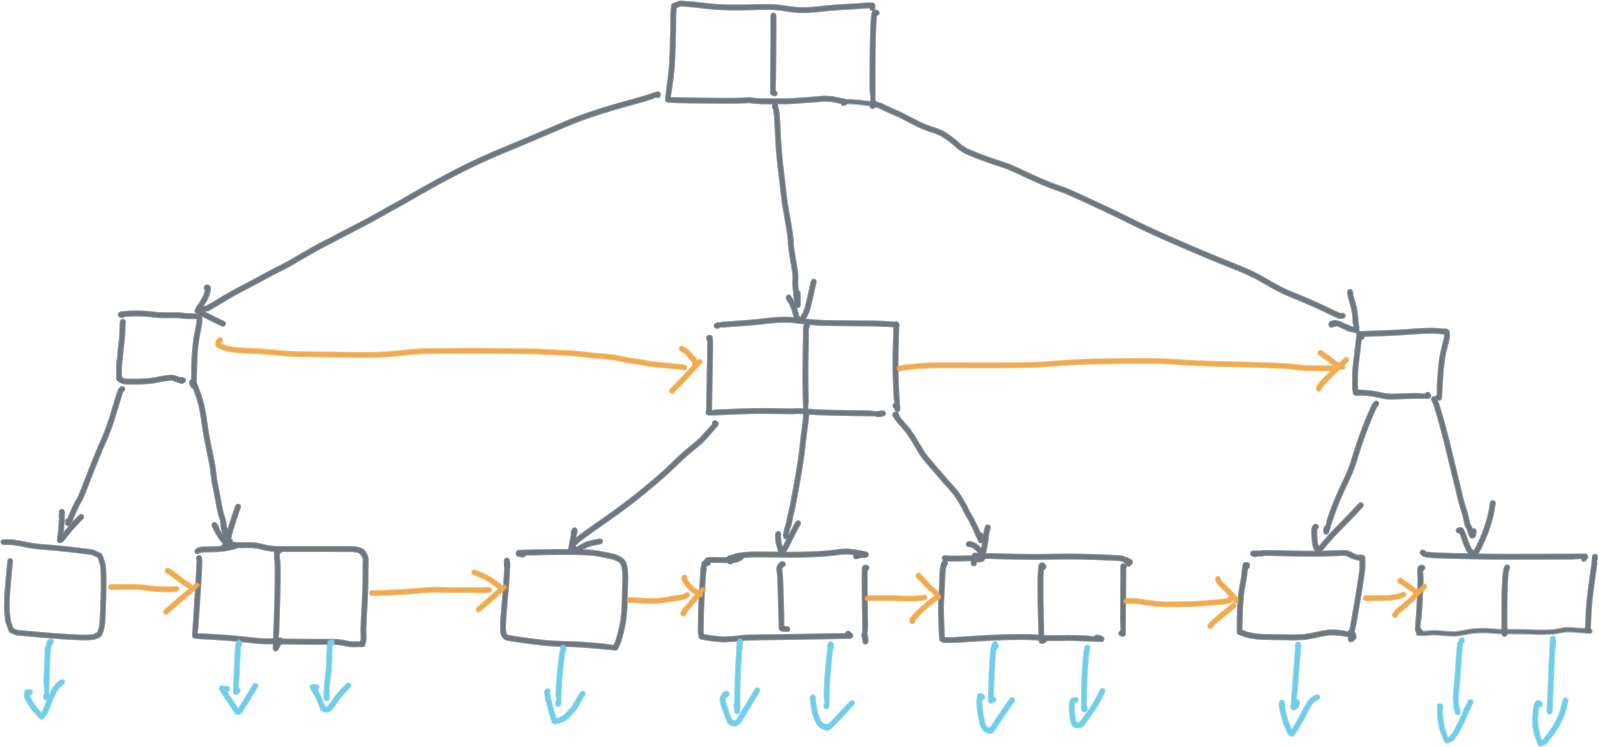
\includegraphics[width=\textwidth]{components/figure/b-link-tree.png}
  \caption{B-Link-Tree with $Order$ = 3}
  \label{figure:b-link-tree}
\end{figure}

Splitting during node insertion is divided into two independent steps: splitting a node and inserting the split node with its new separator key to the parent node. When splitting node $x$, a new right sibling node $y$ is created. The node $y$ inherits the high key from the split node $x$, whereas the first key of $y.keys$ is used as a new $x.highkey$. Thus, an internal node does exist without a parent in between the operations. $x.highkey$ is used to be able to traverse the newly split node and its subtree, even when the split operation is not complete.

\todo{Add insertion pseudocode}

As the final step of node splitting, the separator key and the newly split node $y$ are inserted in the parent node.

\todo{Add search pseudocode}

Tree traversal is modified to honor $x.highkey$ by returning the node at $x.sibling$ when the target key $k$ is larger or equal than $x.highkey$.

\todo{Add interaction correctness proof}

\subsection{Proof of correctness}

To prove the correctness of each operation performed on the B-link-tree, the following theorems need to be proven:

\begin{itemize}
  \item \textit{Deadlock freedom} -- threads performing operations on the B-link-tree cannot produce a deadlock,
  \item \textit{Correct tree modifications} -- the tree must appear as a valid tree for all nodes at any time,
  \item \textit{Correct interactions} -- concurrent operations do not interfere with one another.
\end{itemize}

\begin{theorem}
  \textit{Deadlock freedom} -- threads performing operations on the B-link-tree cannot produce a deadlock.
\end{theorem}

\begin{proof}
  By imposing a total ordering of nodes, cycles are eliminated from the system and thus the system is deadlock free.

  To prove a total ordering of nodes, the following ordering $a < b$, where $a$ and $b$ are nodes of the tree, is considered:

  \begin{enumerate}
    \item If $a$ and $b$ are not on the same distance from the root node, then $a < b$ if and only if node $a$ is less distant from root node than node $b$ (bottom-up).
    \item If $a$ and $b$ are on the same level, then $a < b$ if and only if node $b$ is reachable from node $a$ by following a chain of one or more $sibling$ pointers (left-to-right).
  \end{enumerate}

  It can be shown that during insertion operation the total ordering of nodes is preserved. If $a < b$ at time $t_0$ at the start of insertion, then $a < b$ is preserved for $\forall t, t > t_0$, as a node $x$ during split operation will create a node $x^\prime$ and $x^{\prime\prime}$, where $x^\prime < x^{\prime\prime}$ and:

  $$\forall y, y < x \Leftrightarrow y < x^\prime$$
  $$\forall y, x < y \Leftrightarrow x^{\prime\prime} < y$$

  Therefore, insertion will not break the total ordering of nodes.

  Latches for the nodes are acquired by following the ordering, thus once a latch is acquired for a node, no other latch will be acquired on any node below it, nor on any node on the same level.
\end{proof}

\begin{theorem}
  \textit{Correct tree modifications} -- the tree must appear as a valid tree for all nodes at any time.
\end{theorem}

\todo{Complete proof}

\begin{proof}
  The tree must appear as a valid tree for all threads at any time except for the modifying thread. Splitting happens atomically and writing happens only in three circumstances:
  - writing to a non-full node - ok
  - writing to a newly allocated   node - ok, no pointers are there
  - writing to a split node - atomic transaction needs to happen to transfer the state of node
\end{proof}

\begin{theorem}
  \textit{Correct interactions} -- concurrent operations do not interfere with one another.
\end{theorem}

\todo{Complete proof}

\begin{proof}
  We need to prove that concurrent operations do not interfere with one another. Reader/writer and writer/writer do not step on each other.

  Prove a case of colliding insertion and search operation. We need to consider the case of search operation before insertion is complete (eg: search operation S reads node n insertion operation I modifies the node from n to n', search operation S continues with contents based on n).

  Three types of split:
  - simple insertion of value/pointer pair
  - splitting of a node, insertion to the left (same) node
  - splitting of a node, insertion to the right (new) node

  Simple insertion into a non-full node. Leaf nodes are trivial, internal nodes inserting a pair. Newly inserted node can be acceseed via the side pointers.

  Search while split. If searching in a node mid-split, the search stays the same except for the newly inserted node, which won't be found. If searching in an internal node, \todo{Explain, why nodes below the split node are correct}.

\end{proof}

